\documentclass[a4paper,12pt]{article}
%For links
%\usepackage{url}
%For images
\usepackage{graphicx}
\begin{document}
\begin{enumerate}
    \item $$sin(2x)=0.875$$
          Med en miniräknare tar man $sin^{-1}$ på båda sidorna och räknar ut
          $$2x=sin^{-1}(0.875)\Rightarrow x=sin^{-1}(0.875)/2\approx 0.533$$

          Så för alla blir det ungefär $0.533+2\pi n, n\in \mathbf{Z}$.
          Rent geometriskt kan det beskrivas nedan.
          Det gör det även självklart
          att det andra svaret inom $0 \leq x \leq \pi$ är $\pi-x\approx=2,61$ som ligger till vänster om bilden.

          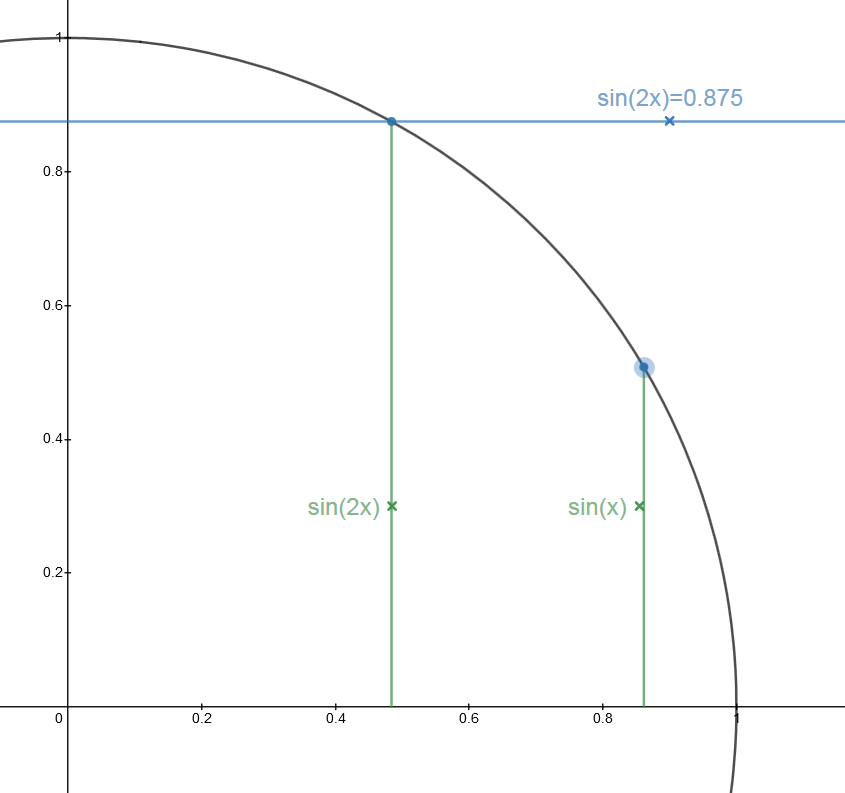
\includegraphics[scale=0.45]{Figur1.png}

    \item
          \begin{enumerate}
              \item Med ren spekulation, 2.5 är mindre än pi men mer än pi/2, så det måste vara i andra kvadranten.
                    Vi vet att $\pi=180^\circ $. Vi kan nu ta fram det med
                    hjälp av enhetsanalys. Om 180 är grader per radie, och pi är endast ett nummer, och v är en vinkel
                    i grader, så kommer vi få $v\pi / 180$ som svar. Räknar man ut enheterna får man radien.

              \item Vi sätter in det som v i ekvationen och vi får $36\pi / 180 = 9 \pi/ 45$
          \end{enumerate}

    \item
          \begin{enumerate}
              \item Man kan rita $y=cos(2x)$ genom att tänka sig en pendel som åker igenom cirkeln dubblet
                    så snabbt som den vanliga pendulen. Då kommer varje vinkel x nås dubbelt så snabbt. Då blir
                    cos(2x) för 45 graders vinkeln $\pi/4=0$. Vid $\pi/2$ är det då -1 osv.

                    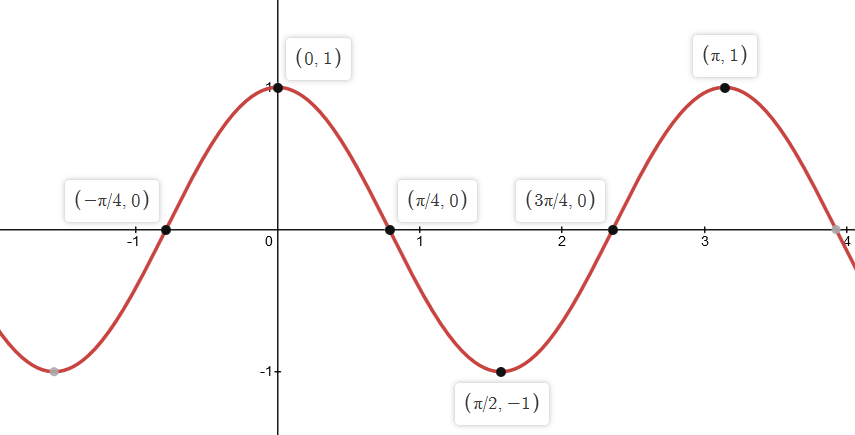
\includegraphics[scale=0.5]{Figur2.png}

              \item Det första man kan ta reda på är noll punkterna. Detta sker vid $\pi/6$ och $7\pi/6$,
                    eller generellt vid $(1+6n)\pi/6$.
                    Detta är för att $pi/6$ i ekvationen är fas skiften som skiftar vart pendeln börjar.
                    Maxpunktens x-position kommer ligga vid genomsnittet
                    av nollpunkterna dvs $\frac{\pi/6+7\pi/6}{2}=\frac{8\pi}{12}=\frac{2\pi}{3}$, och eftersom
                    amplituden är 3 så kommer y-positionen vara 3. Då får vi grafen

                    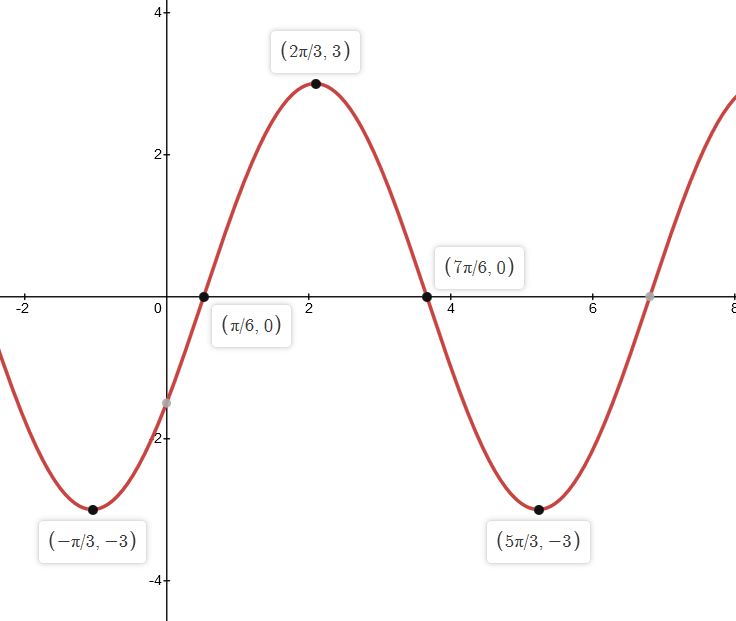
\includegraphics[scale=0.5]{Figur3.png}
          \end{enumerate}

    \item Börja med att dela båda sidorna med sin(x)
          $$2cos(x)=1$$
          $$cos(x)=1/2$$
          Detta sker vid $60\deg$ så svaret är 60 grader.

    \item \begin{enumerate}
              \item Cos är som störst vid t=0 så
                    $$\max_{t}(3+1.5cos(0.1\pi t))=4.5$$
              \item
                    $$3+1.5cos(\pi t/10)=4$$
                    $$cos(\pi t/10)=2/3$$
                    $$t=10cos^{-1}(2/3)/\pi \approx 2.7$$
                    Grafiskt:

                    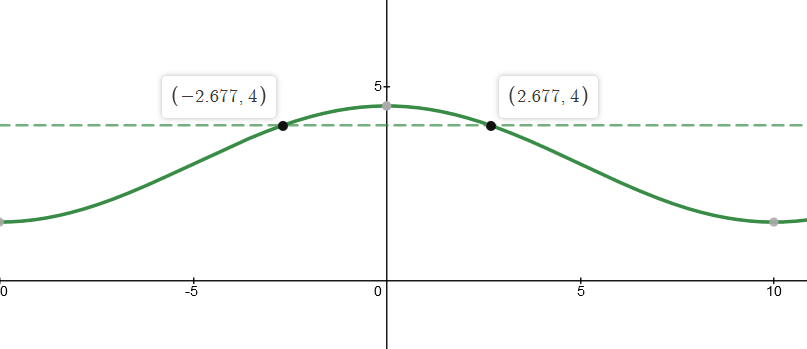
\includegraphics[scale=0.5]{Figur4.png}

          \end{enumerate}

    \item fun
\end{enumerate}
\end{document}